\label{sec:DETRavenApproach}
The main subject of this report is to explain the newer Adaptive Dynamic Event Tree (ADET) methodology developed within the RAVEN code. As already mentioned, the DET approach is extremely effective (achiving almost a perfect tradeoff) with respect to computational resources usage and the effective exploration of the uncertain domain (input space). The proposed approach is designed to further focus these features of the DET methodology toward the characterization of some properties of the input space. More specifically, the approach that will be introduced is an adaptive methodology that defines the branching strategy in order to identify more efficiently (lower computational costs) and more accurately the location of transitions in the input space (e.g., failure vs. success). The characterization of the input space is translated into an “optimization-like” problem for the identification of the so-called Limit Surface, and accelerated through the employment of artificial intelligence-based algorithms that help the selection of future branching points.

The concepts mentioned here in brief are explained in detail in the following sub-sections.
%%%%%%%%%%%%%%%%%%%%%%%%%%%%%%
\subsection{Concept of Limit Surface }
%%%%%%%%%%%%%%%%%%%%%%%%%%%%%%
\label{sec:LimitS}
 As already mentioned, the adaptive methodology can be considered as a goal oriented sampling strategy for the research of the limit surfaces (LSs). To define the meaning of the LS, it is necessary to introduce the concept of “goal” function. Without making a rigorous mathematical treatment, the “goal” function is an object that is defined as a part of the system outcome space. In a safety context, the goal function usually represents the success or failure (transition) of the system. Therefore, if $\overline{x}_{f}$ is the final status of the system, $C\left (\overline{x}_{f}\right )$ the goal function ( $C\left (\overline{x}_{f}\right ) = 1$ system success,  $C\left (\overline{x}_{f}\right ) = -1$ system failure), ), it is possible to define $\overline{x}_{f,L}$ as the transition surface in the output space with respect to the goal function. This statement can be translated in the following mathematical expression: $\overline{x}_{f,L} = \left \{ \overline{x}_{f}|\left | \overline{\bigtriangledown} C\left ( \overline{x}_{f} \right ) \right |= \infty \right \}$. If $\overline{x}\left (t,\overline{p},\overline{x}_{0}  \right )$ represents the evolution of the system (that can be considered deterministic, once the initial condition ($\overline{x}_{0} $) and stochastic model parameters ($\overline{p}$) have been chosen), then is it possible to identify the set of pairs $\left ( \overline{p},\overline{x}_{0} \right )_{LS}$, in the input space, which leads the system outcome to match $\overline{x}_{f,L}$. Such set of points $\left ( \overline{p},\overline{x}_{0} \right )$ represents the limit surface, in the input space.The LS represent therefore the boundary between inputs leading to success or failure of the system, and more generally boundaries among transition regions.

Since the probability of a particular outcome is equivalent to the probability of being in the input space that leads to that outcome, the probability of a system outcome (e.g. success/failure) can be evaluated by computing the probability of being in the space surrounded by the LS.
The determination of the LS is extremely important since its informative content.  Its knowledge: allows to efficiently evaluate risk functions, informs regarding which uncertainties are the most relevant from a risk point of view (ranking of uncertain space), defines safe regions to be explored for plant optimization, identifies risk neutral design direction, etc. Unfortunately, the determination of LSs is very computationally expensive, since a brute-force approach would imply the evaluation of each point of an N-dimensional grid that discretizes the input space. The number of points in this grid is proportional to the requested accuracy. In order to overcome these limitations, a possible approach is the employment of acceleration schemes based on Reduced Order Models (ROMs). ROMs are used to predict the location of the LS in order to drive the exploration of the input space toward its possible location. The Adaptive Dynamic Event Tree is based on this concept.
\label{sec:ADET}
\begin{figure}[h]
  \centering
     \includegraphics[width=0.8\textwidth]{figures/DET_LS_pb.png}
  \caption{Dynamic Event Tree Limit Surface}
  \label{fig:LSDET}
\end{figure}
%%%%%%%%%%%%%%%%%%
%%%%%%%%%%%%%%%%%%%%%%%%%%%%%%
\subsection{Reduced Order Models}
%%%%%%%%%%%%%%%%%%%%%%%%%%%%%%
\label{sec:ROMs}
As mentioned in the previous section, the Adaptive Dynamic Event Tree uses ROMs in order to accelerate the search of transition boundaries represented by the LS. Simplistically, a ROM is a mathematical model of fast solution trained to predict a response of interest of a physical system. The training process is performed by “sampling” the response of a physical model with respect to variations of parameters that are subject to probabilistic behavior. The results (outcomes of the physical model) of those samplings are fed into the algorithm representing the ROM that tunes itself to replicate those results. More specifically, in RAVEN case the reduced order model is constructed to emulate a numerical representation of a physical system. In fact, as already mentioned, the physical system model would be too expensive to be used to explore the whole input space, exploration that would be needed for the limit surface search. Under certain assumptions, the ROM ability to predict the output space of a system improves, increasing the number of training samples (better representation of the whole domain).  This is not always true, since some of the ROMs used might be subject to over-fitting issues.
In RAVEN, several different Reduced Order Model types are available, such as Support Vector Machine, Neighbors based, multi-class models, Quadratic Discriminants, etc. All those supervised learning algorithms have been imported via an Application Programming Interface (API) within the scikit-learn~\cite{scikitlearn} library.

The acceleration schemes in the adaptive approach use a class of supervised learning algorithms usually referred to as “classifiers.” In essence, classifiers are ROMs specialized to represent a binary response of a system (e.g., failure/success, on/off, etc.), like the goal function of interest in our case.
%%%%%%%%%%%%%%%%%%%%%%%%%%%%%%%%%%%%%%%%%%%%%%%%%%%%%%%%%%%%%%%%%%%%%%%%%%%%%%%%
%%%%%%%%%%%%%%%%%%%%%%%%%%%%%%
\begin{figure}[h]
  \centering
     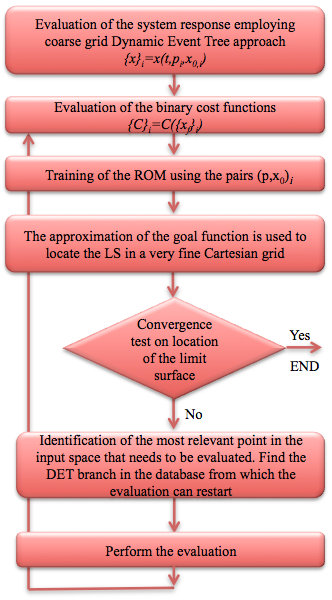
\includegraphics[width=0.5\textwidth]{figures/AdaptiveDET.png}
  \caption{Adaptive Dynamic Event Tree Scheme}
  \label{fig:AdaptiveDET}
\end{figure}
\subsection{Adaptive DET}
%%%%%%%%%%%%%%%%%%%%%%%%%%%%%
The main idea of the application of the previously explained adaptive sampling approach to the DET comes from the observation that the DET is intrinsically adaptive.

In order to explain this statement, as an example, fig.~\ref{fig:LSDET} shows a LS generated by the DET sampling methodology currently available in RAVEN. In this case, a goal function based on the clad max temperature has been used:
\begin{equation}
\left \{ C \right \}_{i}=\left \{ \begin{matrix}
1 & T_{C,i}\geq T_{C,F}\\
-1 & T_{C,i}<  T_{C,F}
\end{matrix} \right.
\end{equation}
where $T_{C,i}$ is the clad temperature and $T_{C,F}$ is the failure temperature, sampled by triangular distribtuion.
As it can be seen, the DET method, when one or more uncertain parameters directly influence the outcome of the goal function, tends to search for the LS with accuracy equal to the user defined grid discretization in the input space.
For this reason, it appears natural to use the DET approach to perform a goal-function oriented pre-sampling of the input space. The proposed approach can be described through the following steps (see Figs.~\ref{fig:AdaptiveDET}~\ref{fig:ADETflowChart}):
\begin{enumerate}
\item A limited number of points in the input space $\left ( \overline{p},\overline{x}_{0} \right )_{i}$ are selected via a DET approach
\item The system code is then used to compute all the possible evolution of the system starting from the above selected input points:
\begin{equation}
    \overline{x}_{i}=\overline{x}\left (t,\overline{p}_{i},\overline{x}_{0,i}  \right )
\end{equation}
\item The goal function  $C\left (\overline{x}_{f}\right )$ (in this case of type Boolean) is evaluated at the final phase space coordinate of the system (outcome):
\begin{equation}
 \left \{ C \right \}_{i}=\left \{ \overline{x} \left (  t=t_{end},\overline{p}_{i},\overline{x}_{0,i}\right )\right \}
\end{equation}
\item The set of pairs $\left ( \overline{p},\overline{x}_{0} \right )_{i} \rightarrow \left \{ C \right \}_{i}$ are used to train a ROM
\item The ROM is used to predict the value of the goal function on a regular Cartesian grid  in the domain space. The grid meshing is dictated by the user-requested accuracy in the determination of the LS location:
\begin{equation}
 \begin{matrix}
 \left \{ c \right \}_{j} \cong ROM\left ( \left \{ \overline{x}_{0} \right \}_{j} \right ) & j=1,...,M
\end{matrix}
\end{equation}
where $j=1, ..., M$ points on the grid
\item The regions identified by a change in value of $\left \{ c \right \}_{j}$ (between -1 and 1) are therefore the ROM prediction of the limit surface location:
\begin{equation}
(\overline{p},\overline{x}_{0})_{LS}
\end{equation}
\item The position of the LS is compared with the one at the previous iteration; if no changes are consecutively detected for a user-defined number of times than the iterations stop; otherwise a new point, in the input space, needs to be selected to increase the ROM training set.
\item The next selected point to be added to the training set is the one located on the limit surface that is the farther from all the other already selected points
\item A hierarchical searching process is performed on the DET branches already evaluated and the starting point (branch) for the new evaluation is determined
\item The process restart from point 2.
\end{enumerate}
\begin{figure}[h]
  \centering
     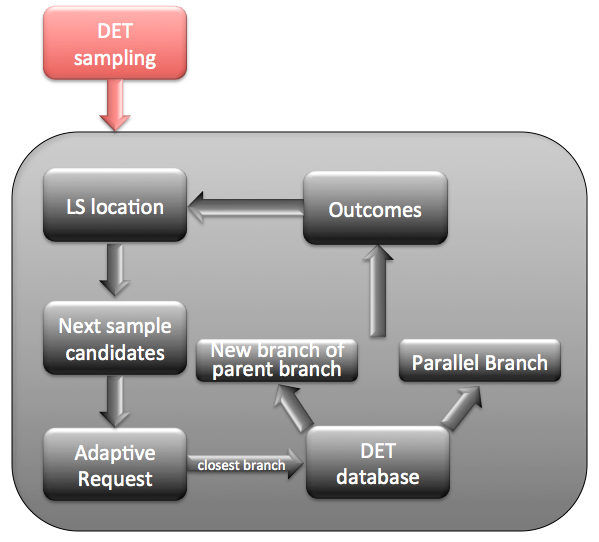
\includegraphics[width=0.6\textwidth]{figures/adaptiveFlowChart.png}
  \caption{Dynamic Event Tree Flow Chart}
  \label{fig:ADETflowChart}
\end{figure}

In order to understand how the algorithm works, it is necessary to explain in details the first and ninth steps of the previous algorithm flow. The ADET methodology starts with a standard DET that performs the initial exploration of the input space, exploiting its capability to investigate the uncertain domain in a reasonably short time. As already mentioned and shown in fig.~\ref{fig:LSDET}, when a goal function is directly influenced by one (or more) uncertain parameter(s), the DET tends to increase the sampling density in proximity of the transition boundaries (LS). This means that the acceleration ROM gets trained with an initial dataset closed to the LS that reasonably helps the convergence of the method.

After the initial DET, the actual adaptive scheme starts to be employed following the calculation flow previously reported. Every time a new point, in the input space, is requested, a search in the DET database is performed. This search is needed to identify the closest branch with respect to the next point needs to be evaluated. Once the closest branch has been identified, the system code is run using that branch as starting point (i.e. the calculation restarts from an advanced point in time). This new evaluation is then added to the DET database and can be used for sub-sequential requests. This approach speeds the adaptive search up and employs an effective exploration of the input space in proximity of the transition boundaries.

In essence this methodology combines the adaptive search algorithm already present in RAVEN with a DET approach, allowing the re-usage of branches of simulations already performed rather than restarting the simulation always from the begin.



